\section{语义模型}
\label{sec:semantic-model}

\begin{frame}
  \begin{center}
    \Huge{\textcolor{red}{语义模型}}
  \end{center}
\end{frame}

\subsection{语义模型}

\begin{frame}[fragile]{语义模型}
  \begin{c++}
Rule:    int -> String
Matcher: int -> boolean
Action:  int -> String
  \end{c++}
\end{frame}

\begin{frame}[fragile]{匹配器}
  \begin{c++}
Matcher: times | contains | always
  \end{c++}  
\end{frame}

\begin{frame}[fragile]{执行器}
  \begin{c++}
Action: to | nop
  \end{c++}  
\end{frame}

\begin{frame}[fragile]{规则库}
  \begin{block}{规则库}
  \begin{c++}
Rule: atom | allof | anyof
  \end{c++}  
  \end{block}

  \begin{block}{隐式树}
  \begin{c++}
atom: (Matcher, Action) -> String
allof(rule1, rule2, ...): rule1 && rule2 && ... 
anyof(rule1, rule2, ...): rule1 || rule2 || ...
  \end{c++}  
  \end{block}  
\end{frame}

\begin{frame}[fragile]{DSL}
  \begin{figure}
    \centering
    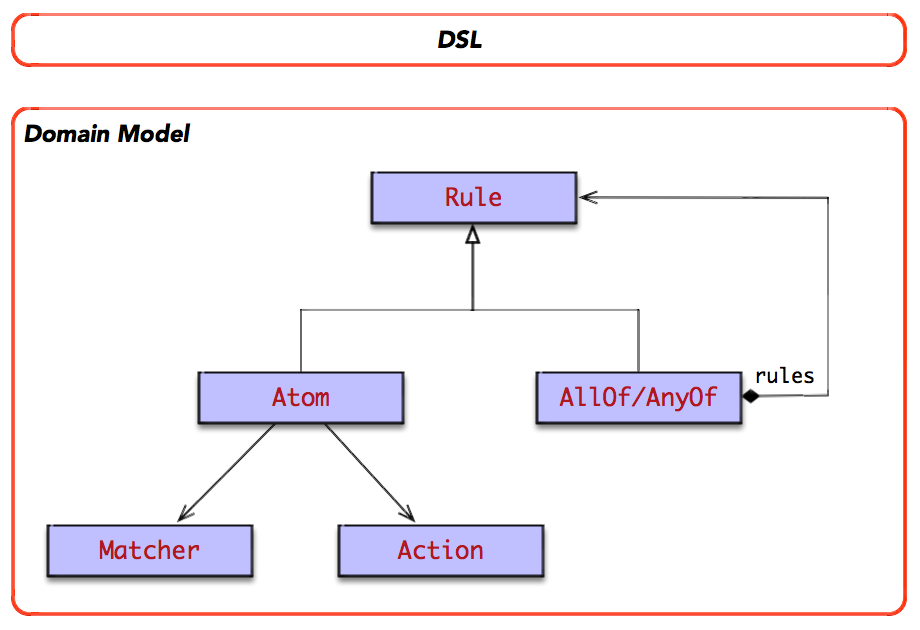
\includegraphics[width=0.8\textwidth]{domain.png}
  \end{figure}
\end{frame}
